% Options for packages loaded elsewhere
\PassOptionsToPackage{unicode}{hyperref}
\PassOptionsToPackage{hyphens}{url}
%
\documentclass[
]{book}
\usepackage{amsmath,amssymb}
\usepackage{lmodern}
\usepackage{ifxetex,ifluatex}
\ifnum 0\ifxetex 1\fi\ifluatex 1\fi=0 % if pdftex
  \usepackage[T1]{fontenc}
  \usepackage[utf8]{inputenc}
  \usepackage{textcomp} % provide euro and other symbols
\else % if luatex or xetex
  \usepackage{unicode-math}
  \defaultfontfeatures{Scale=MatchLowercase}
  \defaultfontfeatures[\rmfamily]{Ligatures=TeX,Scale=1}
\fi
% Use upquote if available, for straight quotes in verbatim environments
\IfFileExists{upquote.sty}{\usepackage{upquote}}{}
\IfFileExists{microtype.sty}{% use microtype if available
  \usepackage[]{microtype}
  \UseMicrotypeSet[protrusion]{basicmath} % disable protrusion for tt fonts
}{}
\makeatletter
\@ifundefined{KOMAClassName}{% if non-KOMA class
  \IfFileExists{parskip.sty}{%
    \usepackage{parskip}
  }{% else
    \setlength{\parindent}{0pt}
    \setlength{\parskip}{6pt plus 2pt minus 1pt}}
}{% if KOMA class
  \KOMAoptions{parskip=half}}
\makeatother
\usepackage{xcolor}
\IfFileExists{xurl.sty}{\usepackage{xurl}}{} % add URL line breaks if available
\IfFileExists{bookmark.sty}{\usepackage{bookmark}}{\usepackage{hyperref}}
\hypersetup{
  pdftitle={Cresko Laboratory Manual},
  pdfauthor={Cresko Lab},
  hidelinks,
  pdfcreator={LaTeX via pandoc}}
\urlstyle{same} % disable monospaced font for URLs
\usepackage{longtable,booktabs,array}
\usepackage{calc} % for calculating minipage widths
% Correct order of tables after \paragraph or \subparagraph
\usepackage{etoolbox}
\makeatletter
\patchcmd\longtable{\par}{\if@noskipsec\mbox{}\fi\par}{}{}
\makeatother
% Allow footnotes in longtable head/foot
\IfFileExists{footnotehyper.sty}{\usepackage{footnotehyper}}{\usepackage{footnote}}
\makesavenoteenv{longtable}
\usepackage{graphicx}
\makeatletter
\def\maxwidth{\ifdim\Gin@nat@width>\linewidth\linewidth\else\Gin@nat@width\fi}
\def\maxheight{\ifdim\Gin@nat@height>\textheight\textheight\else\Gin@nat@height\fi}
\makeatother
% Scale images if necessary, so that they will not overflow the page
% margins by default, and it is still possible to overwrite the defaults
% using explicit options in \includegraphics[width, height, ...]{}
\setkeys{Gin}{width=\maxwidth,height=\maxheight,keepaspectratio}
% Set default figure placement to htbp
\makeatletter
\def\fps@figure{htbp}
\makeatother
\setlength{\emergencystretch}{3em} % prevent overfull lines
\providecommand{\tightlist}{%
  \setlength{\itemsep}{0pt}\setlength{\parskip}{0pt}}
\setcounter{secnumdepth}{5}
\usepackage{booktabs}
\usepackage{amsthm}
\makeatletter
\def\thm@space@setup{%
  \thm@preskip=8pt plus 2pt minus 4pt
  \thm@postskip=\thm@preskip
}
\makeatother
\ifluatex
  \usepackage{selnolig}  % disable illegal ligatures
\fi
\usepackage[]{natbib}
\bibliographystyle{apalike}

\title{Cresko Laboratory Manual}
\author{Cresko Lab}
\date{2021-04-29}

\begin{document}
\maketitle

{
\setcounter{tocdepth}{1}
\tableofcontents
}
\hypertarget{the-cresko-lab}{%
\chapter{The Cresko Lab}\label{the-cresko-lab}}

Description of our laboratory

\hypertarget{introduction-to-the-lab}{%
\chapter{Introduction to the Lab}\label{introduction-to-the-lab}}

\begin{figure}
\centering

\includegraphics{images/Lab_logo.png}
\caption{Illustration by Dr.~Allison Fuiten}
\end{figure}

We are an intellectual community of geneticists who specializes in quantitative evolutionary genomics. Our laboratory studies the developmental genetic and genomic basis of evolution in natural populations. We use the threespine stickleback and zebrafish as the main animal models in the laboratory, as well as syngnathid. We have produced some of the first work that has helped develop stickleback into a model for dissecting the genetic basis of natural variation. We have developed genomic tools such as sequenced Restriction site Associated DNA (RAD) tags that help geneticists apply Next Generation Sequencing (NGS) technologies to biomedical and evolutionary genetic problems. These techniques allow for the efficient identification of thousands of single nucleotide polymorphisms (SNPs) throughout the genomes of models and non-model organisms. We produced the first SNP whole genome-scan for selection in the stickleback genome, and we developed novel Maximum Likelihood (ML) analytical tools for NGS data. Computational biologists and computer scientists in our team have produced software packages for genomic analyses that are used by laboratories around the world for the analysis of big data problems. Our laboratory has developed protocols, best practices, and tools for RNA-seq based transcriptomic functional analyses.

\hypertarget{mission-and-vision}{%
\chapter{Mission and Vision}\label{mission-and-vision}}

\begin{figure}
\centering
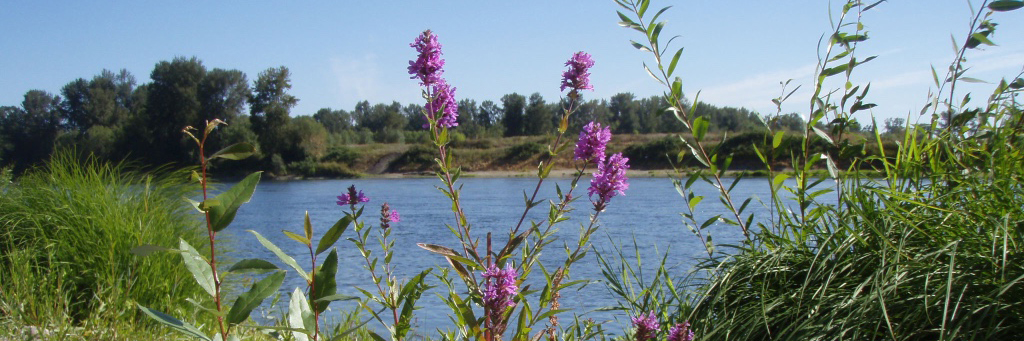
\includegraphics{images/willamette_header.jpg}
\caption{Willametter River}
\end{figure}

We describe our methods in this chapter.

\hypertarget{lab-expectations}{%
\chapter{Lab Expectations}\label{lab-expectations}}

\hypertarget{scientific-ethics-and-integrity}{%
\section{Scientific Ethics and Integrity}\label{scientific-ethics-and-integrity}}

\begin{itemize}
\tightlist
\item
  xx
\item
  xx
\item
  xx
\end{itemize}

\hypertarget{authorship-of-manuscripts}{%
\section{Authorship of Manuscripts}\label{authorship-of-manuscripts}}

\textbf{Recommended: At the start of each project, design your plan for authorship of the project so
everyone knows the expectations}

\emph{Authorship criteria}:

\begin{enumerate}
\def\labelenumi{\arabic{enumi})}
\tightlist
\item
  Makes a significant intellectual contribution to research ideas and experimental design
\end{enumerate}

OR

\begin{enumerate}
\def\labelenumi{\arabic{enumi})}
\setcounter{enumi}{1}
\tightlist
\item
  Makes a significant contribution to data acquisition, data generation, data analysis, data
  interpretation, research coordination, and/or financial support of research
\end{enumerate}

AND

\begin{enumerate}
\def\labelenumi{\arabic{enumi})}
\setcounter{enumi}{2}
\tightlist
\item
  Contributes to writing part of the manuscript, in addition to editing revisions before
  submission for publication
\end{enumerate}

AND

\begin{enumerate}
\def\labelenumi{\arabic{enumi})}
\setcounter{enumi}{3}
\tightlist
\item
  Remains involved throughout the submission and revision process until final publication
\end{enumerate}

*Research participants not meeting the criteria should be listed in the Acknowledgments
section of the final published manuscript

\emph{Authorship order}:

Generally, the person who had the most significant contribution to the project and who does
most of the writing will be the first author. In ecology, the last author is generally the PI of the
lab (although not always). The remaining authors are usually listed in their order of
contribution. However, if contributions were equivalent, then co-authors can be alphabetized
or ordered according to their time since involvement in the project.

\hypertarget{cresko-lab-safety-protocols}{%
\chapter{CRESKO LAB SAFETY PROTOCOLS}\label{cresko-lab-safety-protocols}}

\textbf{FOR YOUR OWN SAFETY AND THE SAFETY OF OTHERS, HEED THE FOLLOWING RULES!}

EMERGENCY CONTACT: dial 911 first, \emph{AND} 6-2919 (EHS) \textbar{} Mark Cell 541-505-0006

\textbf{•} **Safety Shower, Eyewash, Fire Extinguishers. Eyewashes must be flushed weekly. \emph{Undergraduate research assistants are responsible for flushing the safety showers each week.} \_Each lab member is responsible for knowing the locations of safety showers and fire extinguishers in the lab. Safety showers and fire extinguishers are tested annually by EHS.

\hypertarget{wear-a-lab-coat-and-closed-toed-shoes-when-working-with-the-following-chemicals}{%
\section{\texorpdfstring{Wear a lab coat** \textbf{and closed-toed shoes} \textbf{when working with the following chemicals:}}{Wear a lab coat** and closed-toed shoes when working with the following chemicals:}}\label{wear-a-lab-coat-and-closed-toed-shoes-when-working-with-the-following-chemicals}}

\begin{itemize}
\item
  organics (e.g.~phenol/chloroform, Trizol, DNAzol, formaldehyde, formamide, methanol)
\item
  strong acids and bases
\end{itemize}

\hypertarget{wear-eye-protection-when-working-with}{%
\section{\texorpdfstring{Wear** \textbf{eye protection} \textbf{when working with:}}{Wear** eye protection when working with:}}\label{wear-eye-protection-when-working-with}}

\begin{itemize}
\item
  UV light (UV opaque glasses/face shield)
\item
  phenol/chloroform, strong acids/bases, and any splash hazard with anything hazardous in it.
\end{itemize}

\hypertarget{wear-safety-gloves-when-working-with-any-of-the-reagents-above.}{%
\section{Wear safety gloves when working with ANY of the reagents above.}\label{wear-safety-gloves-when-working-with-any-of-the-reagents-above.}}

Heed the ``one glove rule'': remove one glove when moving between rooms to avoid touching doorknobs with a contaminated glove. Note that glove materials differ in their permeability to different reagents. Standard nitrile gloves are adequate for our lab's standard procedures. However, if you are planning experiments that involve more dangerous reagents, consult with Luke Sitts at EHS to select appropriate gloves.

\hypertarget{disposal-of-common-hazardous-reagents-ehs-disposal-6-3192}{%
\section{Disposal of common hazardous reagents (EHS DISPOSAL: 6-3192)**}\label{disposal-of-common-hazardous-reagents-ehs-disposal-6-3192}}

\begin{itemize}
\item
  E. coli plates and recombinant materials: autoclave buckets or EHS biohazard incineration boxes
\item
  E. coli flasks/liquids: bleach, rinse, drain
\item
  Used alcohols, formaldehyde, and kit waste: waste containers under the thermocyclers.
\item
  organic solvents: waste bottles in hood.
\end{itemize}

\hypertarget{storage-of-hazardous-liquids}{%
\section{\texorpdfstring{Storage \textbf{of Hazardous Liquids}}{Storage of Hazardous Liquids}}\label{storage-of-hazardous-liquids}}

\begin{itemize}
\tightlist
\item
  Store flammables and strong acids in a latched METAL SAFETY CABINET UNDER THE HOOD.
\end{itemize}

\hypertarget{heating-liquids-in-the-microwave-oven}{%
\section{Heating Liquids in the Microwave Oven**}\label{heating-liquids-in-the-microwave-oven}}

Triple check that the cap is \emph{very} loose or (better) remove it entirely. Remelting of gels with DNA binding dyes is forbidden.

\hypertarget{bunsen-burners}{%
\section{Bunsen Burners**}\label{bunsen-burners}}

\begin{itemize}
\item
  Triple check that the gas is shut completely off before you leave the bench/ hood.
\item
  keep burners far away from any flammable liquids.
\end{itemize}

\hypertarget{liquid-nitrogen-and-dry-ice}{%
\section{Liquid Nitrogen and Dry Ice**}\label{liquid-nitrogen-and-dry-ice}}

\begin{itemize}
\item
  Use only in well ventilated spaces to avoid asphyxiation.
\item
  Never store in sealed containers to avoid explosions
\item
  Wear lab coat, gloves, goggles. In case of frostbite or burn, soak affected part in tepid water, seek medical attention
\end{itemize}

\hypertarget{lone-worker-guidelines-for-laboratory-personnel}{%
\chapter{LONE WORKER GUIDELINES FOR LABORATORY PERSONNEL}\label{lone-worker-guidelines-for-laboratory-personnel}}

The UO Laboratory Safety Advisory Committee (LSAC) feels that working alone in laboratories should be discouraged but recognizes that a prohibition would hinder the research and education missions of the UO. To advance personnel safety while also recognizing research needs, the LSAC developed this guidance document to assist lab workers in recognizing dangers and developing appropriate procedures.

The primary danger in working alone is that if an accident should occur, there will be delays in rendering aid.

Before working alone, you should:

\begin{enumerate}
\def\labelenumi{\arabic{enumi}.}
\tightlist
\item
  Ensure that you have been trained on the procedures, reviewed the safety data sheets for all associate materials, and know the emergency procedures for your lab.
\item
  Consider whether the risk outweighs the benefits of working alone.
\item
  Consider whether this work can be done at a time when others are around.
\item
  Consider using a buddy system with individuals in other labs nearby.
\end{enumerate}

If you decide to proceed with hazardous procedures on your own, please use a check-in or text-in system with supervisors or peers, ensuring that they know where and when this work is done and that they have contact information readily available for campus safety personnel.

SPECIFIC GUIDELINES FOR THIS LABORATORY

Examples of materials and procedures in THIS laboratory that should be avoided while working alone are provided below. Should you choose to do lone work of this nature, ensure that others know where and when this work will be performed, and when it is completed.

Building \& Room: \emph{Pacific 310 \& 324}\_\_ Supervisor: \_\_Dr.~William Cresko\_

In this laboratory these chemicals or procedures will not be used or done while working alone:

The use of phenol chloroform and the movement of glass aquariums will not be done while working alone in Pacific 310 or 324.

In this laboratory, these procedures will not be conducted while working alone:

Procedures that require the use of phenol chloroform or the movement of glass aquariums

Other safety considerations for working alone in this laboratory (add pages as needed):

Emergencies -- Dial 911
Lab Safety Coordinator:
Safety and Risk Services/EHS: 541-346-3192

\hypertarget{iacuc}{%
\chapter{IACUC}\label{iacuc}}

descriptions of animal care IACUC protocols

\hypertarget{recipes}{%
\chapter{Recipes}\label{recipes}}

\begin{figure}
\centering
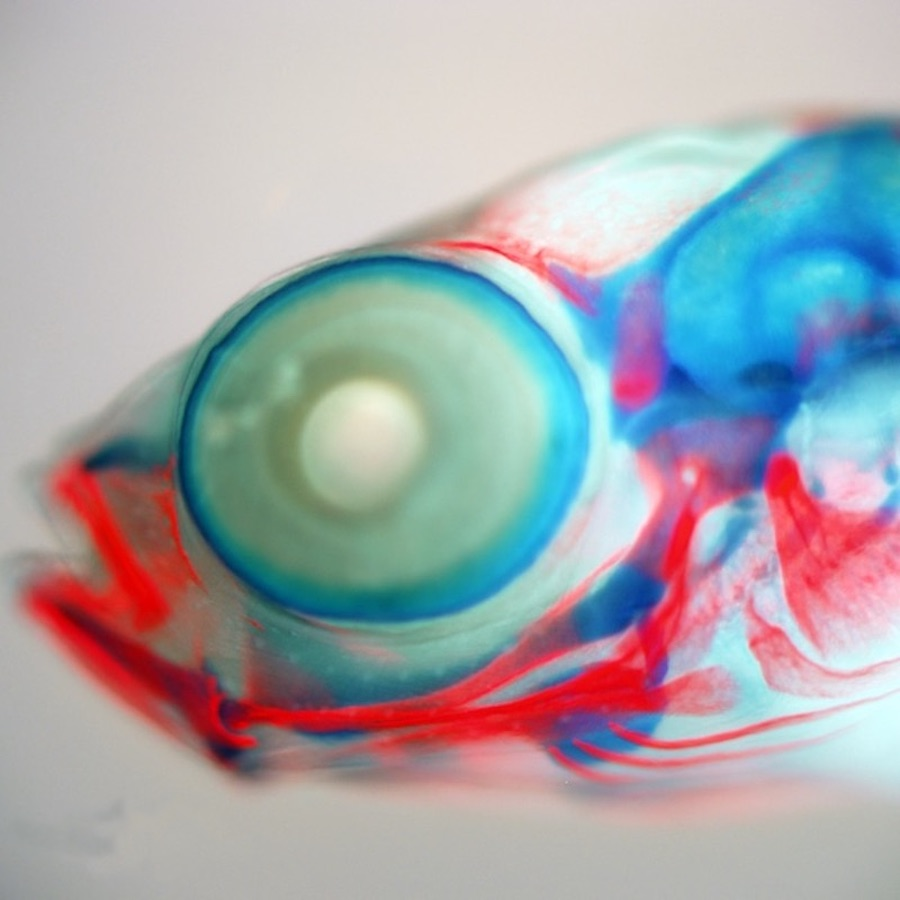
\includegraphics{images/double_head.jpg}
\caption{Photo by Mark Currey}
\end{figure}

\begin{center}\rule{0.5\linewidth}{0.5pt}\end{center}

\hypertarget{embryo-medium}{%
\section{Embryo Medium}\label{embryo-medium}}

\hypertarget{material-needed}{%
\subsection{Material Needed:}\label{material-needed}}

\begin{itemize}
\tightlist
\item
  Instant Ocean Salt
\item
  Baking Soda
\item
  npH2O
\end{itemize}

\hypertarget{embryo-medium-solution}{%
\subsection{Embryo Medium solution:}\label{embryo-medium-solution}}

\begin{enumerate}
\def\labelenumi{\arabic{enumi}.}
\tightlist
\item
  Add 8g Instant Ocean to 2 liters of npH2O
\item
  Add \textasciitilde0.5g baking soda
\item
  Check pH and adjust to 7.0 -- 8.0
\item
  This makes 2 liters
\end{enumerate}

\begin{itemize}
\tightlist
\item
  Salt and baking soda are located in containers near the dissecting scope. Rinse 2 liter flasks with DI water between uses.
  \_\_\_\_\_\_\_\_\_\_\_\_\_
\end{itemize}

\hypertarget{mesab}{%
\section{MESAB}\label{mesab}}

\emph{Tricaine must be pharmaceutical-grade. We use tricaine purchased from Pentair, manufactured by Western Chemical and FDA approved. Tricaine (3-amino benzoic acid ethyl lester also called ethyl m-aminoboenzoate) comes in a powdered form. Purchase the smallest amount possible because tricaine expires quickly.}

\hypertarget{material-needed-1}{%
\subsection{Material Needed:}\label{material-needed-1}}

\begin{itemize}
\tightlist
\item
  Mesab, a.k.a. MS222, tricaine, or 3-aminobenzoic acid ethyl ester
\item
  1 M Tris (pH 9)
\item
  DD water
\end{itemize}

\hypertarget{mesab-stock-solution-4gl-tris-buffered}{%
\subsection{Mesab Stock Solution (4g/L) (tris buffered):}\label{mesab-stock-solution-4gl-tris-buffered}}

\begin{itemize}
\item
  \begin{enumerate}
  \def\labelenumi{\arabic{enumi}.}
  \tightlist
  \item
    4 g tricaine powder
  \end{enumerate}
\item
  \begin{enumerate}
  \def\labelenumi{\arabic{enumi}.}
  \setcounter{enumi}{1}
  \tightlist
  \item
    979 ml DD water
  \end{enumerate}
\item
  \textasciitilde21 ml 1 M Tris (pH 9)
\item
  Adjust pH to \textasciitilde7\\
\item
  Aliquot in 50ml tubes, label with MESAB Stock Solution 4g/L, and store in a -20 freezer
\item
  This makes 1 liter of solution.
\end{itemize}

\hypertarget{euthanasia-solution-300-mgl}{%
\subsection{Euthanasia Solution (300 mg/L):}\label{euthanasia-solution-300-mgl}}

\begin{enumerate}
\def\labelenumi{\arabic{enumi}.}
\tightlist
\item
  Make a solution of tris buffered Stock Solution as described above. (Or obtain an aliquot from the freezer)
\item
  Combine 7.5ml of stock solution into 100 ml of fish water.
\end{enumerate}

\hypertarget{anesthesia-168-mgl}{%
\subsection{Anesthesia (168 mg/L):}\label{anesthesia-168-mgl}}

\begin{enumerate}
\def\labelenumi{\arabic{enumi}.}
\tightlist
\item
  Make a solution of tris buffered Stock Solution as described above. (Or obtain an aliquot from the freezer)
\item
  Combine 4.2 ml of stock solution into 100 ml of fish water.
\end{enumerate}

\begin{center}\rule{0.5\linewidth}{0.5pt}\end{center}

\hypertarget{testes-storage-solution}{%
\section{Testes Storage Solution}\label{testes-storage-solution}}

\hypertarget{materials-needed}{%
\subsection{Materials Needed:}\label{materials-needed}}

\begin{enumerate}
\def\labelenumi{\arabic{enumi}.}
\tightlist
\item
  NaCl
\item
  KCl
\item
  CaCl2
\item
  NaHCO3
\item
  npH2O
\item
  Gentamycin (antimycotic) (Stock -- 10mg/ml)*
\item
  Cell Culture anti-biotic/mycotic from Gibco-BRL (15240-096) 100x Concentration*.
\end{enumerate}

\begin{itemize}
\tightlist
\item
  Both of these reagents are located in separate boxes in Mark's space in the
\item
  20° C freezer. They are partitioned into 100μl aliquots.
\end{itemize}

\hypertarget{solutions}{%
\subsection{Solutions:}\label{solutions}}

Ginzberg's Ringers
- Mix solids into 750 ml of npH2O
- 6.6g NaCl
- 0.25g KCl
- 0.3g CaCl2
- 0.2g NaHCO3
- Bring to 1 liter total volume with npH2O.
- Store at 4° C.

\hypertarget{testes-solution-100ml}{%
\subsection{Testes solution (100ml)}\label{testes-solution-100ml}}

• Add 100μl of Gentamycin and 100μl of Anti-biotic/mycotic to 100ml of Ginzburg's Ringers solution.
• Store at 4° C.

\hypertarget{pipefish-husbandry-protocols}{%
\chapter{Pipefish Husbandry Protocols}\label{pipefish-husbandry-protocols}}

\begin{figure}
\centering
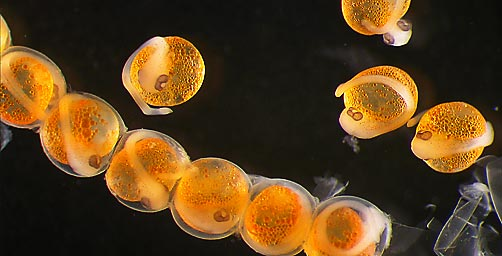
\includegraphics{images/pipefish_embryos.jpg}
\caption{Photo by Mark Currey}
\end{figure}

\begin{center}\rule{0.5\linewidth}{0.5pt}\end{center}

\hypertarget{pipefish-feeding}{%
\section{Pipefish Feeding}\label{pipefish-feeding}}

(created by M Currey 7/23/09)

\textbf{Materials Needed:}

\begin{itemize}
\item
  Decapsualted Brine Shrimp (see artemia decapsulations SOP)
\item
  Adult Brine Shrimp
\item
  Live Moina
\item
  Frozen myisid Shrimp
\item
  Live mysid shrimp
\item
  Shrimp collector
\item
  Squirt Bottle
\item ~
  \hypertarget{fish-foods-for-fry-juvenile-and-adults}{%
  \subsection{Fish foods for fry, juvenile and adults:}\label{fish-foods-for-fry-juvenile-and-adults}}
\item
  Fry - newly hatched baby brine shrimp (see hatching brine shrimp SOP), salt water copepods. Fry are fed once per day
\item
  Adult -- newly hatched brine shrimp, Adult brine shrimp, Moina. Adults are fed once per day. Feed adult brine shrimp when we have them. Use moina when we are out of adult brine shrimp. Adult brine shrimp are from a local fish store and are only available every tow weeks. They last \textasciitilde{} one week and therefore adult pipefish are fed adult brine shrimp for one week and moina the next.
\end{itemize}

\textbf{Fry:}

\begin{verbatim}
     Fry tanks are designated with an orange dot. 
\end{verbatim}

\begin{enumerate}
\def\labelenumi{\arabic{enumi}.}
\tightlist
\item
  Newly hatched brine: Collect newly hatched brine and place into a squirt bottle (see brine shrimp SOP). Feed all tanks with an orange dot.
\end{enumerate}

\textbf{Adults:}

\begin{verbatim}
    Adult tanks are designated with a yellow dot. 
\end{verbatim}

\begin{enumerate}
\def\labelenumi{\arabic{enumi}.}
\tightlist
\item
  Newly hatched brine: Collect newly hatched brine and place into a squirt bottle (see brine shrimp SOP). Feed all tanks with an orange dot.
\item
  Frozen Mysis: Obtain a quarter-sized piece of frozen mysis from the freezer. Place into squirt bottle and add water. Wait until mysis thaws and feed to all adult tanks.
\item
  Adult Brine shrimp: Scoop out adult brine shrimp with net. Wash into a ball and place over the top of squirt bottle. Wash ball of brine into squirt bottle and feed all adult pipefish.
\item
  Moina: Scoop out with net and wash into a ball. Invert ball over collection beaker and wash moina into beaker. Pour moina into squirt bottle and feed.
\item
  Live Mysid: See live foods SOP
\end{enumerate}

\hypertarget{live-food-culture-monia-and-mysid-shrimp}{%
\section{\texorpdfstring{\textbf{Live Food Culture, Monia and Mysid Shrimp:}}{Live Food Culture, Monia and Mysid Shrimp:}}\label{live-food-culture-monia-and-mysid-shrimp}}

\textbf{\emph{Moina}}

\textbf{Materials:}

\begin{itemize}
\tightlist
\item
  10 gallon glass tanks
\item
  corner sponge filter
\item
  Air supply
\item
  Rotifer diet
\item
  Powdered nannochloropsis
\end{itemize}

\textbf{Procedure:}

\begin{itemize}
\tightlist
\item
  Fill 10 gallon tank 3/4 full of stickleback system water
\item
  Add corner filter and activate with air.
\item
  Add Moina
\item
  Change water once every 2-3 weeks by removing half of the water and replacing with stickleback water.
\item
  DO NOT break tank down and clean as moina do not respond well to this.
\end{itemize}

\textbf{Feeding:}

\begin{itemize}
\tightlist
\item
  Add 15 drops of rotifer diet and 1/8 scoop of powdered nannochloropsis each day.
\end{itemize}

\hypertarget{collection-and-feeding-to-fish}{%
\subparagraph{Collection and feeding to fish}\label{collection-and-feeding-to-fish}}

\begin{itemize}
\tightlist
\item
  See pipefish feeding SOP
\end{itemize}

\hypertarget{mysid-shrimp}{%
\subparagraph{\texorpdfstring{\emph{Mysid Shrimp}}{Mysid Shrimp}}\label{mysid-shrimp}}

For a description of the mysid generator please visit:

\url{http://www.mblaquaculture.com/assets/docs/MBL_AQ_Mysid_Generator.pdf}

\textbf{Materials:}

\begin{itemize}
\tightlist
\item
  10 gallon tank generator system
\item
  Salt water
\end{itemize}

\textbf{Feeding:}

\begin{itemize}
\tightlist
\item
  Feed newly hatched brine shrimp daily to both adults and juveniles.
\end{itemize}

\textbf{Water Change:}

\begin{itemize}
\tightlist
\item
  2-3 times per week empty 5 gallons of water from the system and replace with new make up water.
\item
  Make new water in 5 gallon bucket by adding DI water and 2 scoops of salt.
\end{itemize}

\textbf{Juvenile Collection (Daily):}

\begin{itemize}
\tightlist
\item
  Turn off water to tanks.
\item
  Remove collection cup, using mysid system water, rinse juveniles into plastic container.
\item
  Pour juveniles into grow out tank.
\item
  Replace collection cup.
\item
  Turn water on and start siphon.
\end{itemize}

\textbf{Adults collection and feeding to pipefish:}

Juvenile will reach adult size in three weeks. At three weeks these new adults will replace old breeding adults. The old breeding adults that are being replaced are feed to the pipefish.

\begin{itemize}
\tightlist
\item
  Let juveniles grow to three weeks at which point they reach adult stage
\item
  Siphon adults through a net and collect in a container.
\item
  Siphon old adults out of one of the 10 gallon tanks and feed to pipefish
\item
  Clean tank, fill with water and add new adult.
\end{itemize}

\newpage

\hypertarget{live-food-culture-monia-and-mysid-shrimp-1}{%
\section{Live Food Culture, Monia and Mysid Shrimp:}\label{live-food-culture-monia-and-mysid-shrimp-1}}

\textbf{\emph{Moina}}

\textbf{Materials:}

\begin{itemize}
\tightlist
\item
  10 gallon glass tanks
\item
  corner sponge filter
\item
  Air supply
\item
  Rotifer diet
\item
  Powdered nannochloropsis
\end{itemize}

\textbf{Procedure:}

\begin{itemize}
\tightlist
\item
  Fill 10 gallon tank 3/4 full of stickleback system water
\item
  Add corner filter and activate with air.
\item
  Add Moina
\item
  Change water once every 2-3 weeks by removing half of the water and replacing with stickleback water.
\item
  DO NOT break tank down and clean as moina do not respond well to this.
\end{itemize}

\textbf{Feeding:}

\begin{itemize}
\tightlist
\item
  Add 15 drops of rotifer diet and 1/8 scoop of powdered nannochloropsis each day.
\end{itemize}

\hypertarget{collection-and-feeding-to-fish-1}{%
\subparagraph{Collection and feeding to fish}\label{collection-and-feeding-to-fish-1}}

\begin{itemize}
\tightlist
\item
  See pipefish feeding SOP
\end{itemize}

\hypertarget{mysid-shrimp-1}{%
\subparagraph{\texorpdfstring{\emph{Mysid Shrimp}}{Mysid Shrimp}}\label{mysid-shrimp-1}}

For a description of the mysid generator please visit:

\url{http://www.mblaquaculture.com/assets/docs/MBL_AQ_Mysid_Generator.pdf}

\textbf{Materials:}

\begin{itemize}
\tightlist
\item
  10 gallon tank generator system
\item
  Salt water
\end{itemize}

\textbf{Feeding:}

\begin{itemize}
\tightlist
\item
  Feed newly hatched brine shrimp daily to both adults and juveniles.
\end{itemize}

\textbf{Water Change:}

\begin{itemize}
\tightlist
\item
  2-3 times per week empty 5 gallons of water from the system and replace with new make up water.
\item
  Make new water in 5 gallon bucket by adding DI water and 2 scoops of salt.
\end{itemize}

\textbf{Juvenile Collection (Daily):}

\begin{itemize}
\tightlist
\item
  Turn off water to tanks.
\item
  Remove collection cup, using mysid system water, rinse juveniles into plastic container.
\item
  Pour juveniles into grow out tank.
\item
  Replace collection cup.
\item
  Turn water on and start siphon.
\end{itemize}

\textbf{Adults collection and feeding to pipefish:}

Juvenile will reach adult size in three weeks. At three weeks these new adults will replace old breeding adults. The old breeding adults that are being replaced are feed to the pipefish.

\begin{itemize}
\tightlist
\item
  Let juveniles grow to three weeks at which point they reach adult stage
\item
  Siphon adults through a net and collect in a container.
\item
  Siphon old adults out of one of the 10 gallon tanks and feed to pipefish
\item
  Clean tank, fill with water and add new adult.
\end{itemize}

\hypertarget{histological-protocols}{%
\chapter{Histological Protocols}\label{histological-protocols}}

\hypertarget{alizarin-staining}{%
\section{Alizarin Staining}\label{alizarin-staining}}

\hypertarget{purpose-alizarin-staining-of-fixed-adult-stickleback.}{%
\subsection{PURPOSE: Alizarin staining of fixed adult stickleback.}\label{purpose-alizarin-staining-of-fixed-adult-stickleback.}}

\hypertarget{materials}{%
\subsection{MATERIALS:}\label{materials}}

\begin{itemize}
\tightlist
\item
  0.5\% Alizarin red S Stock: To make 50 mls add 0.25g alizarin red S powder to 50 ml water.
\item
  0.025\% Alizarin Stain: To make 100 mls: Add 500µl 0.5\% alizarin red S (stock) to 99.5ml 1\% KOH
\item
  1 Liter: Add 5ml 0.5\% alizarin red S (stock) to 9950ml (1 liter) 1\%KOH
\item
  3\% H202/0.5\%KOH: Mix and keep at 4C; Before using, bring to room temperature to hold down
\item
  introducing bubbles under the skin: 0.5ml 6\%H202 \& 0.5ml 1\%KOH.
\item
  MESAB: Tricaine: 3-amino benzoic acid ethyl ester from Sigma (Cat \# A-5040). Mix in fish safe container with a stir bar:

  \begin{itemize}
  \tightlist
  \item
    400 mg tricaine powder
  \item
    800 mg Na2HPO4 (anhydrous)
  \item
    100 ml glass distilled water
  \end{itemize}
\end{itemize}

Adjust to \textasciitilde pH 7 with a drop at a time of 1N NaOH or 1N HCl if needed
but it's usually right if you weigh the sodium phosphate carefully and
measure the water with a graduated cylinder.

For storage: Aliquot into 6 x 25 ml fish safe plastic bottles and store
at 4C. Label with date made and use within a couple of weeks.

8\% PFA: \{\#pfa .subhead2\}

\begin{itemize}
\tightlist
\item
  8 g Pelleted PFA (Ted Pella, Inc.; cat\# 18501)
\item
  90 ml dH2O
\item
  25 drops 1N NaOH
\end{itemize}

\begin{enumerate}
\def\labelenumi{\arabic{enumi}.}
\tightlist
\item
  Heat at very low heat and stir until solution clears.
\item
  Add 25 drops 1N HCl. pH should be 7.0-7.2.
\item
  Filter and store at 4C not more than 1 week.
\item
  Use as 4\% PFA: dilute 1:1 with 2X PBS, do not store solution more
  than a few hours.
\end{enumerate}

2X PBS \{\#x-pbs .subhead2\}

\begin{itemize}
\tightlist
\item
  1.6\% NaCl
\item
  0.04\% KCl
\item
  0.04 M PO4 pH 7.0- 7.3
\end{itemize}

\hypertarget{procedure}{%
\subsection{Procedure:}\label{procedure}}

Day

Step

Time for Step

Date and Time

1

2h-8h at R/T depending on size on shaker.

1h or longer at R/T on shaker.

Without agitation and with lid open until eyes start to lighten and all
skin pigment is gone (usually about an hour or more)

2

2 h to O/N at R/T on shaker

2 h to overnight O/N at R/T on shaker.\\
Check for bone staining.

R/T on shaker until excess stain in tissue is gone.

Without agitation

Wild caught specimens are put in 100\% EtOH in the field and then
rehydrated and put into 4\% when back in the lab.

  \bibliography{book.bib,packages.bib}

\end{document}
